\section{Project Description}

We developed a system for searching scientific articles.

The data for our search engine is collected from online libraries and from publishers that have information about their articles available online.

% a large number of pages
Firstly, we crawled \texttt{20k} pages from these sources and saved them for future processing.

Then, we filtered irrelevant pages (those that doesn't contain an article description) and processed the rest of the documents.
For each relevant page, we extracted article's title, abstract, list of authors, date of publishing, etc.
Also, we store a link for a PDF version of an article, if it's available.

After that, we implemented a simple search engine for searching among these articles. 

At the end, we collected assessors' evaluations for search results. 
Also, they provided us with feedback on their experience.

\section{System design}
We use \texttt{Python 3}  for development and \texttt{PostgreSQL} database.

Crawlers have own set of sources from where they are allowed to download articles. Also, there is no exchange of URLs between them. The current solution has some advantages over other approaches. For example, scalability. And of course, there are some disadvantages. For more information, see \texttt{DATA ACQUISITION} section.

Articles, processed articles' abstracts and inverted index are stored in a filesystem. To store it in the database is an ineffective approach.
Articles' metadata and PAF are structured data. Thus, they are stored in the database.

We decided to use cos distance for ranking, where vector representations of  articles were built using \texttt{TF-IDF}. It is simple and light solution.

The web interface of our system is implemented using \texttt{Flask} and \texttt{Angular}. \texttt{Flask} is one of the well-known web frameworks for python. It is easy to find documentation and a lot of tutorials. So we decided to use it. 

\texttt{doc2vec} and \texttt{t-SNE} are used for drawing search results on the 2-dimensional plane. It's called article map. We do not use \texttt{word2vec} because it is difficult to build article's vector representation based on vector representations of words the article contains.

To make the evaluation process of search quality easier, we implemented an additional bar with buttons, using which assessors can mark how relevant retrieved documents are.  


\section{Data acquisition}
For data acquisition we implemented a web crawler. \\
The key details of out implementation are:
\begin{enumerate}
    \item
        \textbf{Politeness policy}
        
        We follow the constraints defined in \texttt{robots.txt}.
        We do not visit excluded pages, do not store page if there is a \texttt{noindex} meta tag, and of course, do not spam a website with a lot of queries.
        Even if a delay is not specified in \texttt{robots.txt} we use value defined in the configuration file (default \texttt{delay} is \texttt{50ms}).

    \item
        \textbf{Distributed crawling}
        
        The problem with Python's multithreading is that only one thread can be run at a time because of \texttt{GIL}, so we use multiprocessing instead.
        Each crawler runs in its own process and several crawlers can be run simultaneously.

		Crawlers do not exchange URLs. This solution is suitable in our case because:
		\begin{enumerate}
            \item
                There are not so many data sources with scientific articles so we can just list them.
            \item
            	We are not interested in links leading to another domain, because, most likely, this domain will not contain any relevant documents.
        \end{enumerate}
		\

		Also it gives us a few advantages:
		\begin{enumerate}
			\item Simplicity of implementation. It is more difficult to make a mistake.
			\item Easy to run on different computers, because communication is not needed.
			\item Each crawler has its own set of allowed hosts (we define these hosts in the configuration file). It prevents the same page to be downloaded several times.
		\end{enumerate}

\end{enumerate}

We store each HTML page we crawled in a filesystem and put some page's metadata 
(like its URL, hash of page content, date of last page modify) in database. Duplicated pages (with equal hashes) are ignored.

We crawled articles from \texttt{arxiv.org} and \texttt{springer.com}. But it is not difficult to add new article sources by creating your own parsers. We just have an interface which you need to implement.

\section{Data processing and storage}

As we have a few data sources and we need a specific information extracted from crawled documents
(like article's title, abstract and list of authors), we implemented a separate data processor for each data source.

Data processing is done as follows:
\begin{enumerate}

\item Firstly, we filter out pages that doesn't contain an article.

\item Then, we extract relevant parts of remained pages and transform it to a plaintext, removing all the HTML tags.

\item After that, article's abstract is processed for future indexing, stemming its words and removing stopwords and punctiation

\end{enumerate}

Raw and processed articles' abstracts are stored in the filesystem,
other information (like title, list of authors, link to PDF if available) is put into database.

We use \texttt{BeautifulSoup} for webpage parsing, and \texttt{NLTK} for abstract processing.

\subsection{Indexing}
\subsubsection{Page attribute file}
For each article, we store its attributes: the title, the path to file with abstract, the path to file with processed abstract, the number of words, the link to pdf and so on.

This information we store in the database.

\subsubsection{Inverted index}
We built an inverted index. For each word, we store a list with documents that contain this word. And for each document, we store the number of occurrences of this word in the document with positions of these occurrences.

The document lists are sorted by the number of occurrences. Also, we use gap values to store positions of these occurrences for better compression.

This index can be build by several processes simultaneously. We split all articles by their \texttt{id} into groups, and each group is processed by a separate process. After that, all indices are merged into one index.

We store this index in a filesystem. We use \texttt{gzip} for compression.

\section{Ranking}
We implemented TF-IDF with cosine similarity for ranking.

We used inverted index constructed previously to calculate TF-IDF. 

To improve search perfomance, for each document its vector is constructed once and then stored on disk. 
These vectors are stored in several files, each file contains a batch of vectors.
To decrease memory usage and improve search perfomance even further, vectors are stored in a sparse form.

When answering a query, we retrieve only documents that contain at least one term from the query and then sort them.


\section{Features}
\subsection{Article similarity graph}
We want to plot aricles as points on 2D plane in a way that articles that are ``similar'' would be close to each other as points on plane.

One has an opportunity to see the given documents on this map and click on neighbor articles to open them. 

To measure ``similarity'' of articles we're going to use doc2vec. 
Unfortunatelly, training doc2vec takes some time, so for now we implemented more simple approach.
We use pretrained word2vec to get a vector for each term in an article and then use mean value of these vectors as a document's vector.

Later, we're going to compare this two approaches (but most likely, trained doc2vec would be better)

\subsection{Authors graph}
The same feature will be implemented for authors. 

For each author we'll calculate mean vector of his articles and then visualize it the in same way as for articles.

\section{Interface}
We use \texttt{Flask}, \texttt{Angular} and \texttt{Bootstrap} to visualize search results (fig. 1).

\subsubsection{Additional filters}
Users have an opportunity to search articles not only by content, but also they can specify the date range. In this case, the system shows only that articles which were published in the given date range.

\subsubsection{Articles map}
We project all articles into 2-dimensional space and draw this space. On the map, one can see the extracted documents and click on neighbor articles to open them. It's an additional opportunity to discover similar articles.  

\subsubsection{Feedback}
We decided to add an additional bar with buttons for each retrieved document. Users can use these buttons to mark how relevant the given document is. This feature is a tool for evaluating the performance of our system on the next project stage (fig. 2).

\begin{figure}
  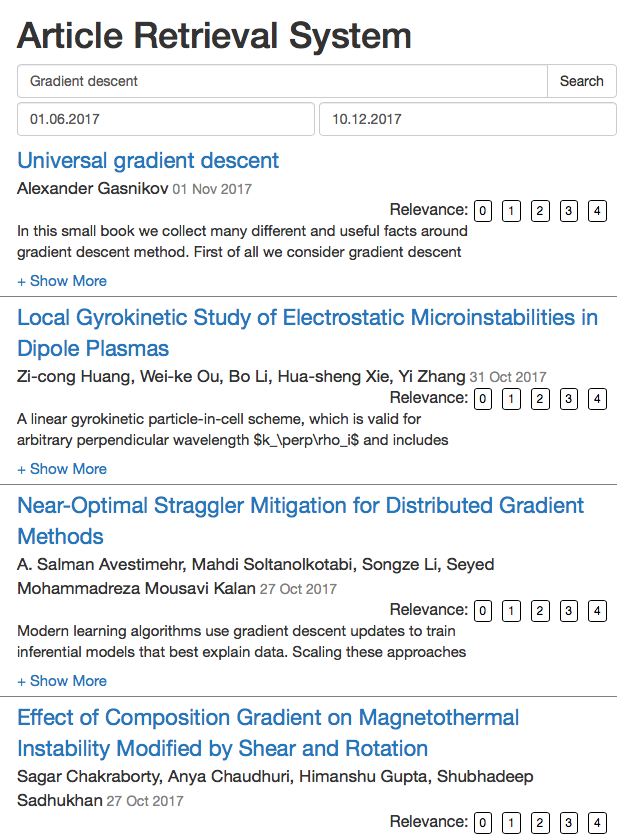
\includegraphics[width=\linewidth]{screenshot_1.png}
  \caption{Search page}
  \label{fig:search_page}
\end{figure}

\section{Evaluation}

We asked 8 assessors to help us evaluate our search service. 

\begin{figure}
  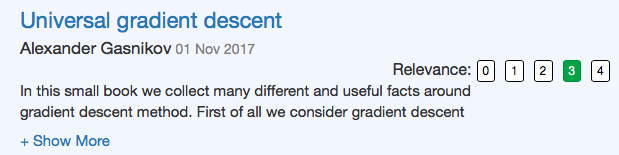
\includegraphics[width=\linewidth]{screenshot_2.png}
  \caption{Feedback tool}
  \label{fig:search_page}
\end{figure}

\subsection{Offline evaluation}
We provided them with 10 search queries listed below in the table and asked them to rank search results on a five-grade scale from 0 (irrelevant) up to 4 (vital document).

Assessors submitted their assessments via search page using evaluation buttons on a search result snippets.

After that, we cleaned up their assessments, removing extra queries and filtering out duplicate assessments for the same query and document rank.
We calculated several metrics based on cleaned assessments: DCG, MAP, RR. We treated document as a relevant if it had average score no less than 2.

\begin{table}
    \centering 
    \begin{tabular}{| l | l | l | l |}
        \toprule
        Query & DCG & MAP & RR \\ 
        \midrule
        gradient descent & 28.078 & 0.833 & 1.000 \\  
        neural networks & 39.942 & 0.917 & 1.000 \\  
        clusterization & 19.989 & 0.639 & 0.500 \\  
        graph theory & 23.480 & 0.450 & 0.500 \\  
        linear differential equations & 15.442 & 0.639 & 0.500 \\  
        numerical analysis & 11.924 & 0.325 & 0.250 \\  
        statistics & 48.747 & 1.000 & 1.000 \\  
        linear programming & 11.905 & 0.250 & 0.250 \\  
        object detection & 26.698 & 0.700 & 1.000 \\  
        music generation & 24.721 & 0.583 & 0.500 \\  
        \bottomrule
    \end{tabular}
    \caption{Search evaluation}
\end{table}

\subsection{Online evaluation}
With our evaluation buttons, users can give us feedback about search quality while using our service.

We store all assessments in the database. So we can calculate different metrics easily.

\subsection{User study}
We asked users about their experience with our search system.

\textbf{Advantages}
\begin{itemize}
	\item Quick article search.
	\item Simple, but nice UI.
	\item Convenient evaluation buttons, which allow accessors to do their job without a headache.
	\item Filters work perfectly.
\end{itemize}

\textbf{Disadvantages}
\begin{itemize}
	\item Keywords are not highlighted.
	\item No additional snippets.
	\item Some articles are in German.
\end{itemize}	
 
\section{Summary}
We designed and developed the system for searching scientific articles from \texttt{arxiv.org} and \texttt{springer.com}. But it is not difficult to add new article sources by implementing your own parsers.

Users can use the system to search articles with specified date range. Also, they are provided with an article map, where search results are highlighted.

Search quality is not bad. We think, that if we download more articles, we will significantly improve it. Especially, if we skip articles written not in English.

\subsection{Future work}
First of all, we need to implement dynamic article map. It will allow users to explore articles more easily and conveniently.

Secondly, it is better to implement multithreading backend. Flask uses single thread by default. 

Also, we can crawl more articles to improve the quality of our search system.

